\subsection{Reduced density matrix (RDM) evaluation algorithm}

High order RDM's are common in post-active space methods that are used
to capture the ``dynamic'' correlation outside of the active space, such as multireference configuration interaction\cite{buenker_individualized_1974} and multireference perturbation theory\cite{andersson_second-order_1990, angeli_n-electron_2002}. 
The expression of quantities in terms of RDM's is a feature of the internally contracted formulations,
which avoid the expansion of the external correction to the active space wavefunction explicitly in terms of many-particle basis states (such as Slater determinants
or configuration state functions). Internally contracted CASPT2\cite{andersson_second-order_1990} and NEVPT2\cite{angeli_n-electron_2002} (both strongly 
and partially contracted variants) require the four-particle RDM, while
 higher levels of correlation can require even higher order RDM's.

In principle, the evaluation of RDM's in DMRG is straightforward; the evaluation of a matrix element such as $\langle \Psi|a^\dag_i a_j |\Psi\rangle$ where $\Psi$
is an MPS, is an operation of $O(k M^3)$ cost and can be carried out 
within any standard DMRG implementation. However, a naive algorithm which 
evaluates each RDM element separately would lead to far too high a computational cost. Instead, the efficient evaluation of the RDM's of an MPS requires forming
suitable intermediates, which takes into account, for example, that the partial trace of an operator $a^\dag_i$ with the wavefunction, over say, the sites left of $i$ in the MPS site ordering, can be reused in {\it all} RDM elements $\langle a^\dag_i a_j \rangle$, where $j$ appears to the right of $i$. Such efficient
algorithms to build the 2-RDM were proposed some years ago by several groups~\cite{ghosh_orbital_2008,zgid_obtaining_2008}, and require only $O(k^3 M^3)$ cost, as opposed to the $O(k^5 M^3)$
cost arising in a naive element by element evaluation. The efficient algorithm to build the 3-RDM was introduced by Kurashige and Yanai in Ref.~\cite{kurashige_second-order_2011}.
Here we introduce a more general algorithm that automatically organises the necessary intermediates for any order of RDM. 
The RDM's we will generally be interested in will be the
spin-summed quantities, e.g. for the 2-RDM, this is
\begin{equation}
\gamma_{ijkl}=\sum_{\sigma,\tau} \bra{\Psi}a^\dagger_{i,\sigma}a^\dagger_{j,\tau}a_{k,\tau}a_{l,\sigma}\ket{\Psi}
\end{equation}


%% Because in DMRG the orbital spaces are partitioned into several blocks, efficient RDM evaluation is not straight forward. The algorithms to build 2-RDM were proposed by several groups. However, they are not feasible for higher order RDM, due to numerous ``cases'' of partitions and types of operators. Here we introduce a general algorithm to generate a loop for every ``case'' and to skip computations for redundant elements automatically.
%% From now on, when we refer a MPS, it means an one-site MPS, because it is needed in evaluation of RDM.
%% The 2-RDM is defined in this way
%% It is similar for the higher order RDM.
%An efficient way to compute RDM elements is to partition operators into left and right block operators as 
%
%\begin{equation}
%  \bra{\Psi} \hat{O}_{LR} \ket{\Psi} = (-1)^P \sum_{l',r',l,r} c^*_{l',r'} \bra{l'}\hat{O}_{L}\ket{l} \bra{r'}\hat{O}_{R}\ket{r} c_{l,r} = Tr(X^TY)
%\end{equation}
%where 
%  $X_{l,r'} =  \sum_{l'} c^*_{l',r'} \bra{l'}\hat{O}_{L}\ket{l} $ , 
%  $Y_{l,r'} =  \sum_{l'}  \bra{r'}\hat{O}_{R}\ket{r} c_{l,r}$
%  and sign $(-1)^P$ is caused by the permutation among the elementary operators and renormalized basis. Computational scaling for $Tr(X^TY)$ operators of $k^{2N}$ RDM elements( k is the number of active orbital and N is the order of the RDM) is $O(k^{2N}M^2)$. The cost for compuation of $X$ and $Y$ depends on how to partition $O_{LR}$ into $O_L$ and $O_R$. In our implementation, we developed a scheme to automatically generate different types of $O_L$ and $O_R$ and the loop to compute RDM elements.
%
%The left block is usually divided into a system block ($\mathcal{S}$), which is expanded during the sweep and the operators on it can be easy build on the flying and a dot block  ($ \mathcal{D}$), where operators is extremely simple and cheap. The right block is the environment-block ($\mathcal{E}$), where operators needed to be precomputed and stored (usually on disk). 


%% It is not affordable to build and store $k^{2N}$ operators used in N-RDM.
%% And for RDM, the expectation value rather than the operators needed. There is no need to build these complicate operators.
%% One efficient way is to distribute the indices (orbital label) $i,j,k,l$ among different orbital subspace for diferent blocks in DMRG.\cite{ghosh_orbital_2008,zgid_density_2008} 
%% The complicate operators are the tensor product of small operators on different blocks. And if small operators are contracted with the wave function before doing tensor product. A dot product rather than the tensor product is needed. It is much cheaper. Below are the details.

\subsubsection{General loop over orbital type patterns and number patterns}

To organize the efficient and non-redundant evaluation of the RDM elements, we label each element in terms of two classifiers: its ``type pattern'' (which describes
the pattern of creation and annihilation operators, ordered by the sites on the lattice), and its ``number pattern'' (which describes how to express
the element in terms of common intermediates). The complete set of RDM elements can be then be obtained efficiently with
proper reuse of intermediates in a DMRG sweep, by looping over all 
type patterns, and all indices corresponding to given number patterns, at each step of the sweep (with a few restrictions associated with edge cases near the ends of the sweep, described in the appendix), building the DMRG renormalized operators corresponding to the given type and number patterns, and forming
the appropriate contractions with the DMRG wavefunction.

The type pattern is precisely defined as follows. Consider an RDM element $\langle {a}^\dagger_i{a}^\dagger_j\dots {a}_m{a}_n\dots \rangle$. 
We reorder the indices such that the indices of the creation and annihilation operators are arranged successively in the order as they appear
in the DMRG site ordering: $\hat{o}_{i'}\hat{o}_{j'}\dots \hat{o}_{m'}\hat{o}_{n'}$, with $i'\le j'\le \dots \le m' \le n'$ and where $\hat{o}$ is either $\hat{a}$ or $\hat{a}^\dagger$.
The corresponding binary pattern of 2$N$ (where $N$ is the rank of the RDM) creation and annihilation operators appearing in the above operator string 
is the ``type pattern'' of the RDM matrix element.

The number pattern encodes how to compute the expectation value $\langle {a}^\dagger_i\hat{a}^\dagger_j\dots \hat{a}_m\hat{a}_n\dots \rangle$
in terms of the DMRG renormalized operators (partial traces of operators with the DMRG wavefunction over a block of orbitals) that
are to be constructed in the DMRG sweep. 
%% Operators like  can be permuted into a form like $\hat{o}_{i'}\hat{o}_{j'}\dots \hat{o}_{m'}\hat{o}_{n'}$, with $i'\le j'\le \dots \le m' \le n'$ and $\hat{o}$ is $\hat{a}$ or $\hat{a}^\dagger$. A string with $N$ $\hat{a}$ and $N$ $\hat{a}^\dagger$ determines the type of the operator. 
%% We call it ``type pattern''. 
%% Then the string is split into several small pieces according to blocks (orbital subgroups) in DMRG sweep. 
Recall that a DMRG sweep consists of a sequence of operations over the orbitals; at each step in the DMRG sweep, there is the set of
orbitals  preceding the current orbital (the system block ($\mathcal{S}$)), the current orbital (the dot block ($\mathcal{D}$)), and the set of orbitals whose
associated site tensors have
yet to be optimized (the environment block ($\mathcal{E}$)). The intermediates in
the  construction of an RDM matrix element
are DMRG renormalized operators  built and stored on the three blocks. 
To determine the renormalized operators to build, we partition the $2N$ orbital labels of the operator $\hat{O}$ 
among the 3 blocks. The most efficient partitioning (when generating
the full set of RDM elements) is to compute a given element from renormalized operators with
the maximum number of orbital labels appearing on the dot block, and an
equal number of  orbital labels on the system and environment blocks. 
For typical RDM elements (i.e. not for elements such as $\gamma_{0000}$), at least one orbital label can be placed on $\mathcal{D}$ and at most $N-1$ orbital labels on $\mathcal{E}$ by choosing an appropriate position of the dot site (i.e. the step in the DMRG sweep). 
The numbers \{$n_\mathcal{S}$,$n_\mathcal{D}$,$n_\mathcal{E}$\} then denote the numbers of orbital labels distributed on the different blocks, and this
is the ``number pattern''. One can generate all valid number patterns, by considering all cases where the number of orbital labels on $\mathcal{S}$ is no more than $N$, that on $\mathcal{D}$ is no more than 4 and that on $\mathcal{E}$ is no more than $N-1$, and the total is $2N$ except for some edge cases for the first step and last step in the sweep, as discussed in the appendix.


%% There are three blocks in a DMRG sweep: the system block  algrithom.
%% The system block ($\mathcal{S}$) is expanded during the sweep and the operators on it can be easy build on the flying. The dot block ($\mathcal{D}$) is composed of a single site and its operators are extremely simple and cheap. The environment block ($\mathcal{E}$) was computed from $\mathcal{S}$ in previous sweep in reverse direction, and its operators needed to be precomputed and stored (usually on disk). 
%% The $2N$ orbital labels of $\hat{O}$ is needed to be partitioned onto the three blocks. It is computational favorable to put more orbital labels on $\mathcal{D}$ and put few orbital labels on $\mathcal{E}$. And the numbers of orbital labels on $\mathcal{S}$ and $\mathcal{E}$ need to be balanced, otherwise number of operators on one block will be extremely big. For most RDM element (not for element like $\gamma_{0,0,0,0}$), at least one orbital label could be put on $\mathcal{D}$ and at most $N-1$ orbital labels on $\mathcal{E}$ by changing the position of the dot site.  

With the above process, the renormalized operators that need to be constructed   on each block $\mathcal{S}$, $\mathcal{D}$, and $\mathcal{E}$ 
in the DMRG sweep, are enumerated
by the corresponding set of ``type patterns'' and ``number patterns'' of the RDM that is being built. In total this leads to $O(k^N)$ renormalized
operators that need to be built, most of which are constructed on the system block $\mathcal{S}$ at different steps in the sweep. The cost to build these operators 
is $O(k^NM^3)$ at each step of the sweep and $O(k^{N+1}M^3)$ in total.   

\begin{figure}\label{fig:operator_split}
  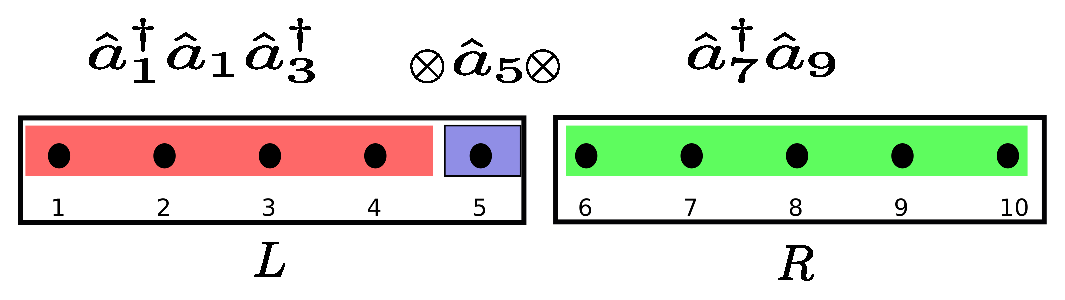
\includegraphics[width=8cm]{operator_split.eps}
  \caption{Evaluation of a three RDM element $\gamma_{1,3,7;1,5,9}$. $\hat{a}_1^\dagger\hat{a}_1\hat{a}^\dagger_3$ is on $\mathcal{S}$, $\hat{a}_5$ is on $\mathcal{D}$, and $\hat{a}^\dagger_7\hat{a}^\dagger_9$ is on $\mathcal{E}$. It belongs to (3,1,2) ``number pattern'' and ($\hat{a}^\dagger\hat{a}\hat{a}^\dagger\hat{a}\hat{a}^\dagger\hat{a}$) ``type pattern''.}
\end{figure}

\subsubsection{Computing the expectation values}

After building the required renormalized operators on the three blocks, $[O]^S$, $[O]^D$, $[O]^E$ at site $i$ of the sweep, they are
traced with the renormalized DMRG wavefunction, i.e. the site tensor $\mathbf{A}^{n_i}$. 
This corresponds to the computation
\begin{align}
\gamma = \sum_{sne} A^{n_i}_{se} p [O]^S_{ss'} [O]^D_{nn'} [O]^E_{ee'} A^{n'_i}_{s'e'} 
\end{align}
where the above tensor contraction is performed in stages (e.g. contracting $s$, $n$, $e$ indices separately) so as to minimize the computational cost,
and $p$ is a parity operation that inserts appropriate minus signs for
fermions~\cite{chan_highly_2002}. The total cost
of this step for the N-RDM is $O(k^{N+1}M^3+k^{2N}M^2)$.


%% combine $\hat{O}^S$ and $\hat{O}^D$ into $O^L$ on the left block, $\mathcal{S}\otimes \mathcal{D}$. (Combining $\mathcal{E}$ and $\mathcal{D}$ only for RDM calcualtions is also feasible.) The $\mathcal{E}$ is the right block.
%%   RDM element $\gamma = \sum_{l,r}\sum_{l',r'} c_{l,r} O^{L}_{l,l'} O^R_{r,r'}c_{l',r'}$ , with $\ket{\Psi} = c_{l,r}\ket{l}\ket{r}$, can be computed in two step. (1) $X_{r,r'} = \sum_{l}\sum_{l'} c_{l,r} O^{l,l'} c_{l',r'}$. (2) $\gamma = \sum_{r,r'} X_{r,r'} O^R_{r,r'}$.
%%   The reason for contracting wave function with $O^L$ first is that the dimension of $O^L$ is $4M$ while the dimension of $O^R$ is $M$.
%%   The number of operation required for forming X is $O(k^{N+1}M^3)$ and that for dot product between $X$ and $O^R$ is $O(k^{2N}M^2)$. 
%%   The computations for N-RDM are 
  %The types of operators on different blocks are also determined automatically. In N-RDM, $N$ $\hat{a}^\dagger$ and $N$ $\hat{a}$ form strings with different orders. They represent different type of $O_{LR}$.
  %The strings are partitioned into three parts according to number of operators in different blocks. This process forms 'patterns' (combinations of different type operators) for the RDM calculations. For exampke, in 2-RDM, for $\hat{a}^\dagger_i\hat{a}^\dagger_j\hat{a}_k\hat{a}_l (i\le j\le k\le l)$ type operators with number of indices partition 2-1-1, all $\hat{a}^\dagger_i\hat{a}^\dagger_j (i\le j)$ operators on $\mathcal{S}$ should be combined with each of $\hat{a}_l$ operators on $\mathcal{E}$ and the only one of $\hat{a}_k$ operator on $\mathcal{D}$. 
  %In order to build operators and corresponding intermedaite ($X$ or $Y$) and to reuse them, operators on $\mathcal{S}$ or $\mathcal{E}$ need to be precomputed and stored. Then do a loop over them. And operators on another block could be built on the fly. 

\subsubsection{Spin recoupling}

Through the above steps, an expectation value such as $\braket{{a}^\dagger_0{a}^\dagger_1{a}_2{a}_3}$ is obtained. 
For a non-spin-adapted DMRG algorithm, where $a^\dag, a$ are simple creation and annihilation operators, 
we can then obtain $\gamma_{0132}$ by permuting $ {a}_2$ and ${a}_3$ with appropriate signs. For spin-adapted DMRG implementations, the $a^\dag, a$ 
are spin tensor creation and annihilation operators, and
$\braket{{a}^\dagger_0{a}^\dagger_1{a}_2{a}_3}$ is a reduced matrix element which generates multiple density matrix 
values through the Wigner-Eckhart theorem.
 The elements generated correspond to $\braket{\{[({a}^\dagger_0{a}^\dagger_1)^{S_1}_{\mathcal{S}}({a}_2)_{\mathcal{D}}]^{S_2}({a}_3)_{\mathcal{E}}\}^{S_3}}$ with different spins $S_1$, $S_2$, $S_3$. The spin tensor creation and annihilation operators can be expanded as a linear combination of spin orbital creation
and annihilation operators, leading to a set of linear equations to obtain the spin orbital RDM elements from a single spin reduced matrix element. Using singlet embedding \cite{tatsuaki_interaction-round--face_2000, sharma_2012}, expectation values for the spin tensor combinations with non-zero total spin are zero, significantly decreasing the number of 
expectation values to compute. The coefficients appearing in the linear equations are the same for all operators with the same pattern and can thus be generated 
automatically and reused. The cost of this process is independent of the DMRG bond dimension $M$, and is thus negligible compared to the other parts of the RDM calculation.
%The spin orbital Nth order RDM elements, solutions of these linear equations, has $(N!)^2$ fold permutation symmetry, much more than correponding spin-averaged RDM's $N!$ fold permuation symmetry, even though the number of element is $2^{2N}$ time of that in spin-averaged RDM.

%The one-particle and two-particle density matrix is defined in this way
%
%\begin{equation}
%\gamma_{i,j}= \sum_\sigma\bra{\Psi}a^\dagger_{i,\sigma}a_{j,\sigma}\ket{\Psi}
%\end{equation}
%\begin{equation}
%\gamma_{i,j,k,l}=\sum_{\sigma,\tau} \bra{\Psi}a^\dagger_{i,\sigma}a^\dagger_{j,\tau}a_{k,\tau}a_{l,\sigma}\ket{\Psi}
%\end{equation}
%
%\subsection{High order particle density matrix}
%Three and four particle density matrix can be used to do multi-reference perturbation calculations. Large number of operators needed in the calculations, high computation scaling and complex spin coupling make the higher order particle density matrix not trivial. We implemented a module to compute different order particle density matrix. It can do loops among different types of operators, pick the non-redundant elements and form linear equations between spin coupling elements and spin average particle density matrix elements, automatically. 
%
%There are $k^8$ elements in four particle density matrix. A trivial way to compute is to compute $<\hat{O}>$($\hat{O}$ has eight indexes) one by one. The scaling is $k^8M^3$. Using intermediate like $\hat{O}[L]\ket{\Psi}$, $\bra{\Psi}\hat{O}[R]$,( a citation), the computation requirement is $O(k^8M^2+k^5M^3)$. It is similar for three particle density matrix. 
%
%Generally, $\hat{O}[L]$ and $\hat{O}[R]$ in four particle density matrix have four indexes. The number of them is $O(k^4)$. It is 
%impossible to store them in the memory in a realistic calculation. They can be divided into different types, based on the number of 
%creation or annihilation operators. Only certain combinations of types of $\hat{O}[L]$ and $\hat{O}[R]$ can have non zero expect value and 
%contribute to results of particle density matrix. One of these combinations are computed at a time. Memory requirement is smaller. 
%
%(Algorithm loops here?)
%
